%%%%%%%%%%%%%%%%%%%%%%%% 
\documentclass[%
	11pt,%
	a4paper,%
	onside,%
	headinclude,%
	footinclude,%
	BCOR5mm,%
	captions=tableheading]%
		{scrartcl}
%%%%%%%%%%%%%%%%%%%%%%%%

%%%%%%%%%%%%%%%%%%%%%%
\usepackage[T1]{fontenc}
\usepackage[utf8]{inputenc}	
\usepackage[french,english]{babel}
%%%%%%%%%%%%%%%%%%%%%%

\usepackage{lastpage} 
\usepackage{mathrsfs}



%%%%%%%%%%%%%%%%%%%%%%%%%%%%%%%%%%%%%%%%%%%%%%%%%%%%%%%%%%%%%%%%%%%
\makeatletter																%
\newif\if@mainmatter														%
\newcommand{\frontmatter}{%												%
  \clearpage																%
  \pagenumbering{arabic}													%
  \edef\computelastpage{%													%
  \uppercase{\the\numexpr\getpagerefnumber{LastFrontPage}-1\relax}}}				%
\newcommand{\mainmatter}{%												%
  \clearpage																%
  \immediate\write\@auxout{\noexpand\newlabel{LastFrontPage}{{}{\arabic{page}}}}%		%
  \@mainmattertrue															%
  \pagenumbering{arabic}													%
  \def\computelastpage{\pageref{LastPage}}}										%
\makeatother																%
%%%%%%%%%%%%%%%%%%%%%%%%%%%%%%%%%%%%%%%%%%%%%%%%%%%%%%%%%%%%%%%%%%%%

\usepackage{amsmath,amssymb}
	
	\renewcommand{\vec}{\mathbf}
	
\usepackage{esint}

\usepackage{indentfirst}

\usepackage{booktabs}

\usepackage{mathtools,amsmath}
	
	\newcommand{\mydef}{\equiv}

\usepackage[separate-uncertainty=true,
	output-decimal-marker={.}]
		{siunitx}

\usepackage[usenames,dvipsnames]{xcolor}
\DeclarePairedDelimiter{\abs}{\lvert}{\rvert}

\usepackage{wrapfig}

\usepackage{sidecap}

\usepackage{lscape}

\usepackage{caption}

\usepackage{subcaption}

\usepackage{lettrine} 

\usepackage{graphicx}

%%%%%%%%%%%%%%%%%%%%%%%%%%%%%%%%%%%%%%%%%%%%%%%%%%
	
\usepackage{pgfplots}
	\pgfplotsset{%
		compat=newest,%
		/pgf/number format/use comma,%
		/pgf/number format/1000 sep={\,},%
		/pgf/number format/min exponent for 1000 sep=4}

%%%%%%%%%%%%%%%%%%%%%%%%%%%%%%%%%%%%%%%%%%%%%%%%%%

%%%%%%%%%%%%%%%%%%%%
\usepackage[%
	nochapters,%
	beramono,%
	eulermath,%
	pdfspacing,%
	listings]%
		{classicthesis}
		

\usepackage{arsclassica}
%%%%%%%%%%%%%%%%%%%%

%%%%%%%%%%%%%%%%%%%%%%%%%%%%%%%%%%%%%%%%%%% head + foot
\pagestyle{scrheadings} 
\clearscrheadfoot
%\chead{\today} 
\ohead[\pagemark]{\thepage\space  of \computelastpage} 
\ihead{\includegraphics[width=.10\textwidth]{EPFL.eps}}
%%%%%%%%%%%%%%%%%%%%%%%%%%%%%%%%%%%%%%%%%%% 

\usepackage{lipsum}
\renewcommand{\sectionmark}[1]{\markright{\spacedlowsmallcaps{#1}}}

%%%%%%%%%%%%%%%%%%%%%%%%%%%%%%%%% margini
\setheadsepline[textwithmarginpar]{2pt}


\paperheight=297mm
\paperwidth=210mm

\setlength{\textheight}{235mm}
\setlength{\topmargin}{-1.2cm} 
%\setlength{\leftmargin}{-1.2cm} 
\setlength{\textwidth}{15cm}
\setlength{\oddsidemargin}{0.56cm}
\setlength{\evensidemargin}{0.56cm}
%%%%%%%%%%%%%%%%%%%%%%%%%%%%%%%%%%

%%%%%%%%%%%%%%%%%%%%%%%%%%%%%%%%%%%%%%	Table of Cont
\usepackage{tocloft}
%\renewcommand{\cftsecleader}{\cftdotfill{\cftdotstep}}
%\renewcommand{\cftsubsecleader}{\cftdotfill{\cftdotstep}}
%\renewcommand{\cftsecdotsep}{\cftdot}
%\renewcommand{\cftsubsecdotsep}{\cftdot}
\renewcommand{\cftsecleader}{\cftdotfill{\cftsecdotsep}}
\renewcommand{\cftsubsecleader}{\cftdotfill{\cftsubsecdotsep}}
%    \renewcommand{\cftdot}{\rule{1pt}{0.4pt}}
    \renewcommand{\cftdotsep}{0}
%%%%%%%%%%%%%%%%%%%%%%%%%%%%%%%%%%%%%%

%%%%%%%%%%%%%%%%%%%%%%%%%%%%%%%%%%%%%%
\newcommand{\mail}[1]{{\href{mailto:#1}{#1}}}
\newcommand{\ftplink}[1]{{\href{ftp://#1}{#1}}}
\newcommand{\httplink}[1]{{\href{http://#1}{#1}}}
%%%%%%%%%%%%%%%%%%%%%%%%%%%%%%%%%%%%%%

%%%%%%%%%%%%%%%%%%%%%%%%%%%%%%%%%%%%% MultiCols
\usepackage{multicol}
\setlength\columnsep{15pt}
\usepackage{setspace}

\usepackage{caption}

% Figures within a column...
\makeatletter
\newenvironment{tablehere}
{\def\@captype{table}}
{}
\newenvironment{figurehere}
{\def\@captype{figure}}
{}
\makeatother
%%%%%%%%%%%%%%%%%%%%%%%%%%%%%%%%%%%%%%


\definecolor{mygray}{gray}{.90}
\definecolor{darkred}{rgb}{0.55, 0.0, 0.0}
\definecolor{darkblue}{rgb}{0.0, 0.0, 0.55}
\definecolor{darkgreen}{rgb}{0.0, 0.2, 0.13}
\definecolor{darkgray}{rgb}{0.66, 0.66, 0.66}
\definecolor{darkgoldenrod}{rgb}{0.72, 0.53, 0.04}

\usepackage{blindtext,wrapfig,calc}
\usepackage{xparse}

%%%%%%%%%%%%%%%%%%%%%% cite
\usepackage[super]{natbib} 
		%%%%%%%%%%%%%%%%%%%%%% caption
\usepackage{setspace}

\captionsetup{format=default,font=small,labelfont={sf,bf}}

		%%%%%%%%%%%%%%%%%%%%%%%%%%%%%%%%%%%%%% MATLAB
\definecolor{mygreen}{RGB}{28,120,0} % color values Red, Green, Blue
\definecolor{mylilas}{RGB}{170,55,241}
\usepackage{listings}

\lstloadlanguages{Matlab}
\lstset{language=Matlab,                        % Use MATLAB
        frame=single,                           % Single frame around code
        basicstyle=\small\ttfamily,             % Use small true type font
        keywordstyle=[1]\color{Blue}\bf,        % MATLAB functions bold and blue
        keywordstyle=[2]\color{Purple},         % MATLAB function arguments purple
        keywordstyle=[3]\color{Blue}\underbar,  % User functions underlined and blue
        identifierstyle=,                       % Nothing special about identifiers
        commentstyle=\usefont{T1}{pcr}{}{sl}\color{mygreen}\small, % Comments small dark green courier
        stringstyle=\color{mylilas},             % Strings are purple
        showstringspaces=false,                 % Don't put marks in string spaces
        tabsize=3,                              % 5 spaces per tab
        %
        %%% Put standard MATLAB functions not included in the default
        %%% language here
        morekeywords={xlim,ylim,var,alpha,factorial,poissrnd,normpdf,normcdf},
        %
        %%% Put MATLAB function parameters here
        morekeywords=[2]{on, off, interp},
        %
        %%% Put user defined functions here
        morekeywords=[3]{FindESS, homework_example},
        %
        morecomment=[l][\color{Blue}]{...},     % Line continuation (...) like blue comment
        numbers=left,                           % Line numbers on left
        firstnumber=1,                          % Line numbers start with line 1
        numberstyle=\tiny\color{Blue},          % Line numbers are blue
        stepnumber=1                        % Line numbers go in steps of 5
        }
%%%%%%%%%%%%%%%%%%%%%%%%%%%%%%%%%%%%%%%%%%%%%

\usepackage{tcolorbox}
\tcbuselibrary{skins}

\usepackage{amsthm}
\newtheorem{definition}{Definition}
\newtheorem{theorem}{Theorem}

\def\Vhrulefill{\leavevmode\leaders\hrule height 0.7ex depth \dimexpr0.4pt-0.7ex\hfill\kern0pt}




%%%%%%%%%%%%%%%%%%%%%%%%%%%%%%%%%%%%%% ABSTRACT

\usepackage{abstract} 
\renewcommand{\abstractnamefont}{\normalfont\bfseries} 
\renewcommand{\abstracttextfont}{\normalfont\small\itshape}

%%%%%%%%%%%%%%%%%%%%%%%%%%%%%%%%%%%%%%



%%%%%%%%%%%%%%%%%%%%%%%%%%%%%%%
%								 %
%	         INIZIO DOCUMENTO          	 %
%								 %
%%%%%%%%%%%%%%%%%%%%%%%%%%%%%%%

\begin{document}

\makeatletter
\renewcommand{\maketitle}{\bgroup\setlength{\parindent}{0pt}
\begin{flushleft}
  \textbf{\@title}

  \@author
\end{flushleft}\egroup
}
\makeatother

\title{\huge{Pattern Classification and Machine Learning}\\[5pt]\textcolor{darkred}{\textbf{\large{\emph{Project : Project 1\\ Supervisor: Gian Franco}}}}}

\author{%
\vspace{10pt}Francesco Cremonesi \footnote{\label{note1}Department of Computer Science PhD, Swiss Institute of Technology Lausanne.}, Riccardo Silini \footnote{Department of Physics MA $3$, Swiss Institute of Technology Lausanne.} - 1 August 1991}

\frontmatter


\maketitle

%%%%%% Abstract Exemple %%%%%%
%\hrule
%\begin{abstract}
%\lipsum[2]
%\end{abstract}
%\hrule

\vspace{.5cm}

\begin{multicols}{2}
%\tableofcontents

%%%%%%%%%%%%%%%%%%%%%%%%%%%%%%%%%%%%%%%%%%%%%%%%%%%%%%%%%%%%
%		DOCUMENT BEGIN
%%%%%%%%%%%%%%%%%%%%%%%%%%%%%%%%%%%%%%%%%%%%%%%%%%%%%%%%%%%%

\section{Preprocessing of data}
We describe the process of removing NaNs, removing cross-correlated features, special treatment of categorical variables and standardization of data.

\subsection{Dealing with NaNs}
As decribed in the CERN document~\cite{cern-doc}, some features may have \emph{missing data} in the form of the value -999.0, which is not valid for any feature.
The approach we test here for dealing with such data is, for each observation in which at least one feature has an invalid value, to remove the whole observation from the dataset.
Applying the process to the training dataset yields a drop in the number of samples of 72\%, i.e. from a total observation count of $2.5 \times 10^5$ to $6.8 \times 10^4$ observations, suggesting that this method is perhaps too consevative.
Surprisingly, not removing the invalid observations yields slightly better solutions in the classification process.
This suggests that it might be worth it to investigate more sophisticated methods of dealing with NaNs, such as assigning missing values to their nearest neighbours.

\subsection{Cross-correlated features}
Some features present a high degree of cross-correlation.
Not only is it more convenient to remove them from a computational point of view, but it can also be better for the numerical stability of some ML algorithms.  \\
%\begin{figure}
%\centering
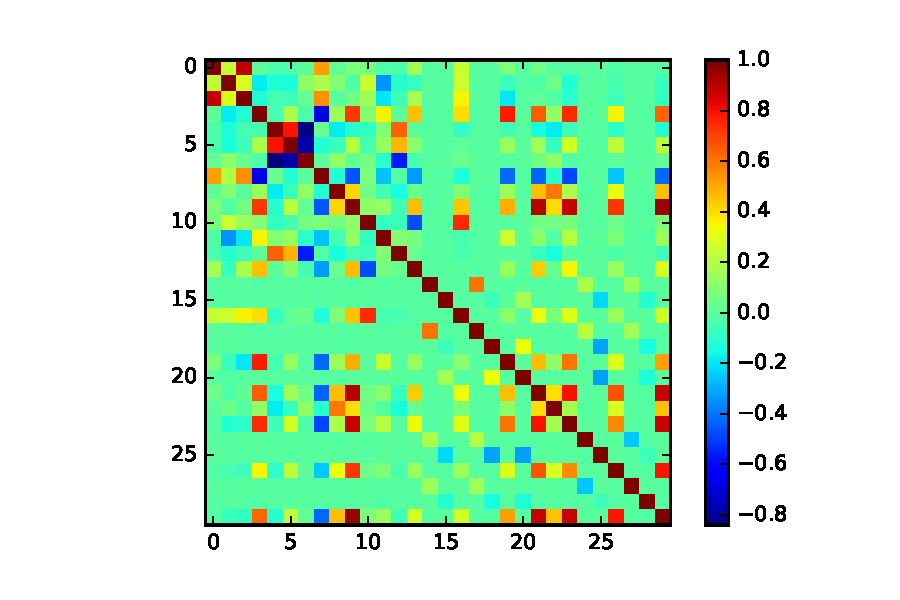
\includegraphics[width=0.8\columnwidth]{corr-coef-matrix.pdf}
\captionof{figure}{Matrix of correlation coefficients. \label{fig-corr}}
%\end{figure}
We analyzed the correlation coefficient matrix in Figure~\ref{fig-corr} and decided to remove feature number 9 (i.e. \texttt{DER\_sum\_pt}) because it is a derived feature with a high correlation ($> 0.95$) to the primary feature number 29 (i.e. \texttt{PRI\_jet\_all\_pt}).

\subsection{Categorical variables}
Analysis of the CERN document~\cite{cern-doc} reveals that one feature, namely \texttt{PRI\_jet\_num}, only takes integer values $0,1,2,3$.
As these represent actual quantities, it is arguable whether this should be treated as a categorical variable or not.
However, since some of the derived features appear to have different formulas according to the value of \texttt{PRI\_jet\_num} we argue that this should be treated as a categorical variable.
As such, we define as customary a set of dummy variables, each one associated to the possible levels of \texttt{PRI\_jet\_num}, that take the value 1 for the observations where \texttt{PRI\_jet\_num} is equal to that level, and 0 otherwise.

\subsection{Standardization of data}
The values taken by different features can vary wildly and take quite large values which can cause overflow problems, thus a normalization procedure is necessary.
We opt for a normalization based on computing the eigendecomposition of the covariance matris of the centered data matrix $X - \bar{X}$:
\begin{equation}
\text{compute } \Lambda, U \text{ such that: } (X - \bar{X}) = U\Lambda U^T.
\end{equation}
This transformation yields the whitened data $X_w$:
\begin{equation}
X_w = \Lambda^{-1/2}U^T(X - \bar{X}).
\end{equation}



%%%%%%%%%%%%%%%%%%%%
%		Introduction
%%%%%%%%%%%%%%%%%%%%

%%%%%% Section Exemple %%%%%%
%\section*{\textcolor{darkred}{Introduction}}
%
%\lettrine[nindent=0em,lines=2]{I}{n} this project we use the tools of \emph{MANO}, a project developed by Luca Randazzo, aiming to help impaired people in the task of closing their hands and for rehabilitation purposes. 
%
%The hardware is composed of a right-hand exoskeleton, as shown in figure [\ref{figurename}], connected through a box containing an Arduino\textsuperscript{\tiny\textregistered}  and mechanical devices, to a EEG cap supporting 16 electrodes. For the EEG recordings, the subject is asked to perform three different tasks: the first is the \emph{EXO} task, in which the exoskeleton mechanically closes the subject's hand, in order to record the brain activation patterns linked to the perception given by the device. This task is also important for the subject's feelings raised by the external device controlling his body. Then it will be asked to perform the so called \emph{MI (Motor intention)} task, in which the subject is asked to imagine the action of closing his hand without actually moving it. The third task, called \emph{MI EXO}, is similar to the \emph{MI} task, but the device will mechanically close the subject's hand regardless of his will. It is asked then, for this last task, to imagine the movement, and once the skeleton closes, to think that it's action is due to the subject's will, which is actually not true. This leads to a difficulty of the task, which should be repeated multiple times in order to have reliable data.

%%%%%% Figure Exemple %%%%%%
%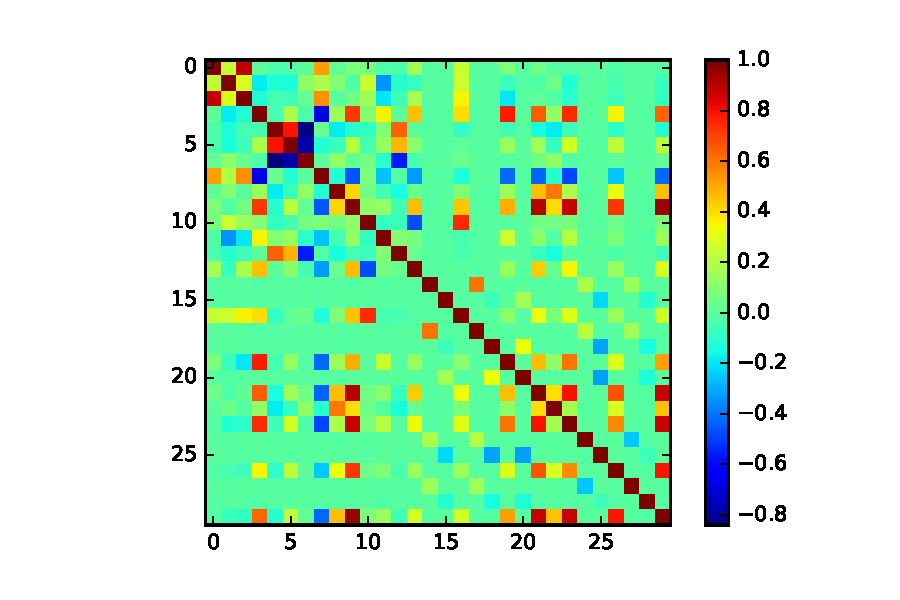
\includegraphics[scale=1]{corr-coef-matrix.pdf}

%%%%%% Table Exemple %%%%%%
%\begin{center}
%\begin{tabular}{  c  c  c  c  } 
% \toprule
%\large{TEST SET}  & $ab10$ & $ac4$ & $ac8$ \\
% \midrule
%MI & $0.576$ & $0.507$ & $0.444$ \\ 
% 
% MIEXO & $0.568$ & $0.235$ & $0.500$ \\ 
% 
% EXO & $0.617$ & $0.188$ & $0.0$ \\ 
% \bottomrule
%\end{tabular}
%\end{center}


\begin{spacing}{0.2}
\small
\begin{thebibliography}{9}

%%%%%% Biblio Exemple %%%%%%
%\bibitem{pfurt} G. Pfurtscheller, J. Kalcher, Ch. Neuper, D. Flotzinger, M. Pregenzer (1996). \emph{Electroencephalography and clincal Neurophysiology, 99, 416-425}.\\
\bibitem{cern-doc} Claire Adam-Bourdarios , Glen Cowan , Cecile Germain , Isabelle Guyon, Balazs Kegl , David Rousseau (2014), \emph{Learning to discover: the Higgs boson machine learning challenge}.\\

 \end{thebibliography}
 \end{spacing}
 

\end{multicols}

\clearpage
\mainmatter
\clearscrheadfoot
\ihead{Figures} 
\pagenumbering{Roman}
\setcounter{page}{1}
\ohead[\pagemark{}]{\pagemark{} of \pageref{LastPage}}  

%\listoffigures
 \clearpage
 
%%%%%% Annex Figure Exemple %%%%%%
%\begin{figure}
%    \centering
%    \begin{subfigure}[b]{0.45\textwidth}
%     \includegraphics[scale=.3]{EPFL.eps}
%        \caption{}
%        \label{fig:13a}
%    \end{subfigure}
%    ~ %add desired spacing between images, e. g. ~, \quad, \qquad, \hfill etc. 
%      %(or a blank line to force the subfigure onto a new line)
%    \begin{subfigure}[b]{0.45\textwidth}
%     \includegraphics[scale=.3]{EPFL.eps}
%        \caption{}
%        \label{fig:13b}
%    \end{subfigure}
%
%
%\caption{$\mathbf{(a)}$: Retrieval error as a function of the flip ratio for $5$ stored patterns. We can see that for a flip ratio below the $30\%$, at convergence we can retrieve exactly the patterns, while above this threshold we have rapid increase of the error, with a large standard deviation. $\bold{(b)}$: Retrieval error as a function of the number of patterns stored with the network for a given flip ratio of $10\%$. We can place the threshold, for which the retrieval error is below $2\%$, at $30$ patterns, while above this threshold we can see an increasing error with big fluctuations. For both figures we chose a network composed of $N=200$ nodes we averaged over $100$ realizations.}
%\end{figure}



\end{document}	
